\subsection{This is a figure}
\subsubsection{Intro}
At times resolution may not match
Images are stored in a matrix.\\
Resturised img\\
vector images do not break.\\
Pdfs are vector. So alphabets do not break\\

\subsubsection{Vector Img}

\begin{figure}[h!]
    \centering
    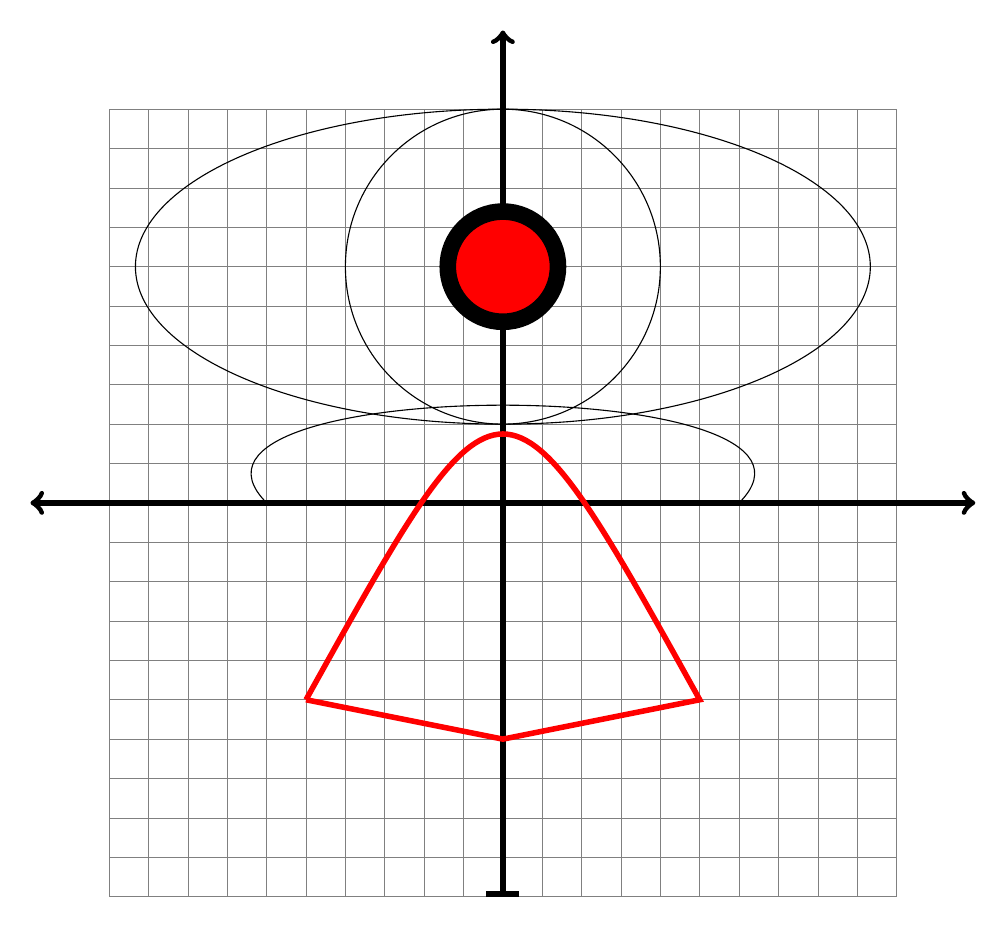
\begin{tikzpicture}[scale=0.5]
        \draw [help lines] (-10,-10) grid (10,10);
      \draw [line width=2pt, <->] (-12,0) -- (12,0);
       
       \draw [line width=2pt, |->] (0,-10) -- (0,12);
       
    %   \draw [red ,line width=2pt, <-> ,rounded corners] (0,0) -- (5,7) -- (-5,7) -- (0,0);
        
        % \draw [blue , line width= 1.2pt , rounded corners] (-5,5) rectangle (4,-4);
        
        % \draw [green,line width= 2.5pt , domain = -3*pi:3*pi, samples = 9000] plot(\x , {5*sin(\x r});
        
        \draw (0,6) circle (4);
        
        \draw [fill = red , line width = 6pt] (0,6) circle (1.4);
        
        \draw [xscale = 7/3] (0,6) circle (4); %Elipse
        
        
        
        % Curve
        \draw [red , line width =2pt ] (-5,-5) .. controls (0,4) .. (5,-5) -- (0, -6) -- (-5 , -5);
        
        \draw (-6 , 0) to [in=45,out=135] (6,0);
          
    \end{tikzpicture}
    
    \caption{Vector Image}
    \label{fig:my_label}
\end{figure}

\subsubsection{Arcs }

\begin{figure}[h!]
    \centering
    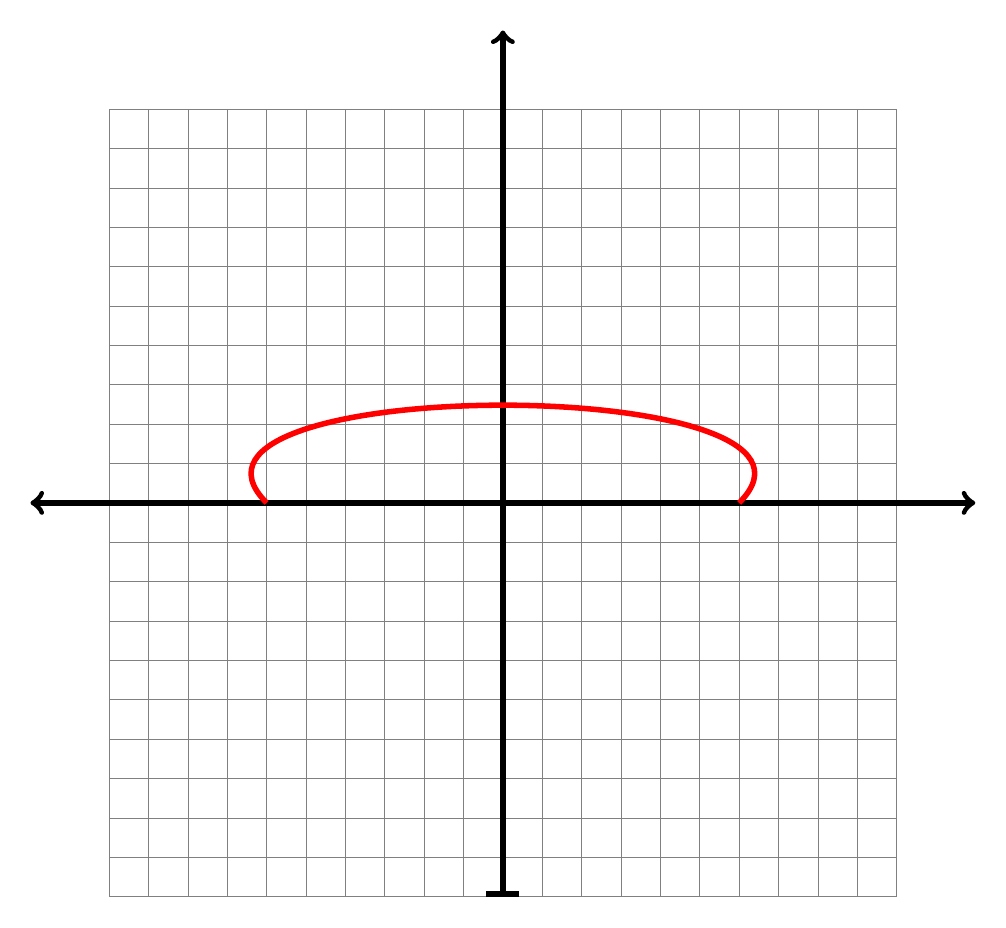
\begin{tikzpicture}[scale=0.5]
        \draw [help lines] (-10,-10) grid (10,10);
      \draw [line width=2pt, <->] (-12,0) -- (12,0);
       
       \draw [line width=2pt, |->] (0,-10) -- (0,12);
       
        \draw [line width=2pt, red] (-6 , 0) to [in=45,out=135] (6,0);
         
        % \draw (-6 , 0) to [in = 45, out = 180] (0 , 7) to [ int = 45,out = 180] (10 ,10); 
          
    \end{tikzpicture}
    
    \caption{Vector Image}
    \label{fig:my_label}
\end{figure}

\subsubsection{Pract}
\begin{figure}[h!]
    \centering
    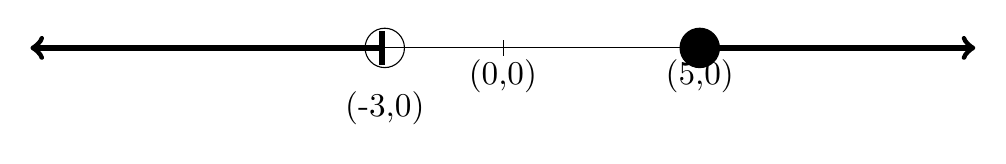
\begin{tikzpicture}[scale=0.5]
        % \draw [help lines] (-10,-10) grid (10,10);
      \draw [line width=2pt, <-|] (-12,0) -- (-3,0);
      \draw [line width=2pt, ->] (5,0) -- (12,0);
       
    %   \draw [line width=2pt, |->] (0,-10) -- (0,12);
       
     \draw  (-3,0) -- (0,0);
     \draw [|-] (0,0) -- (5,0);
    \draw[] (-3 , 0) circle (0.5);
    \draw[fill = black] (5 , 0) circle (0.5);
    \node [scale = 1.2pt, below] at (0 , 0){(0,0)};
    
    \node [scale = 1.2pt, below] at (5 , 0){(5,0)};
    
    \node [scale = 1.2pt, below] at (-3 , -0.8){(-3,0)};
    
    \end{tikzpicture}
    
    \caption{Vector Image}
    \label{fig:my_label}
\end{figure}